\chapter{概率与统计 - 概型、概率和随机变量}

\begin{figure}[ht]
  \centering
  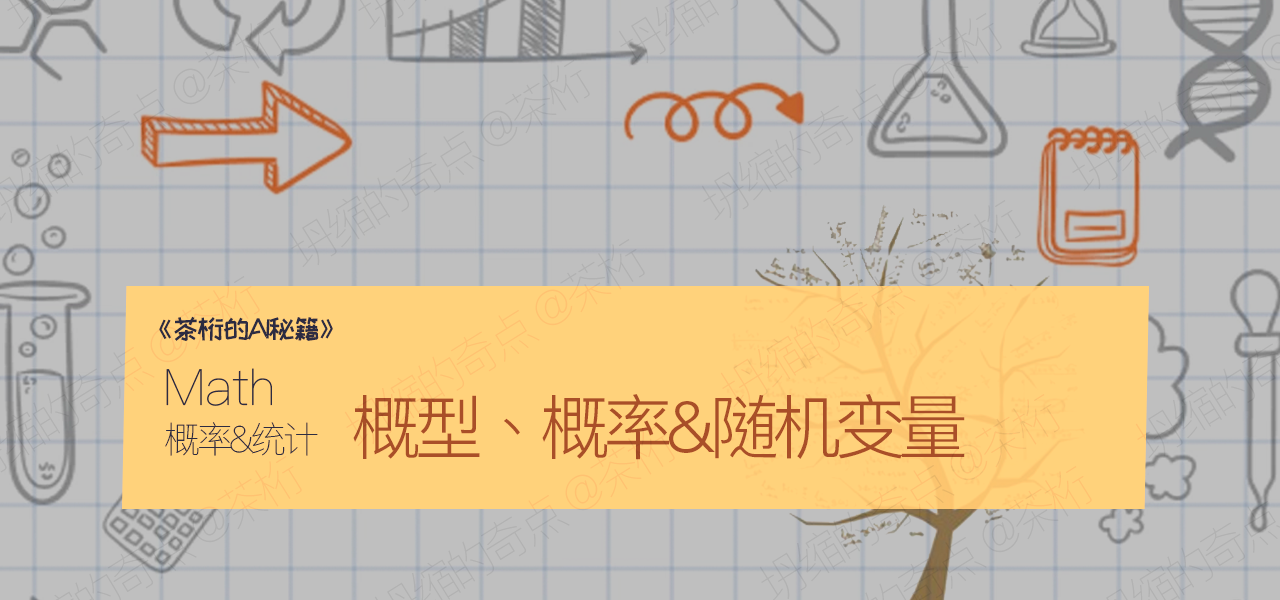
\includegraphics[width=1\linewidth]{asset/茶桁的AI秘籍_Math_20.png}
\end{figure}

\newpage

\section{古典概型}

古典概型其实非常简单, 我们基本上在高中就应该学过这部分内容. 它是我们在概率学习之路上的一个启蒙者, 是我们第一个遇到的一种概率模型. 

首先我们来正儿八经的去看一下它这个定义: 

\begin{newquotation}
若一个随机试验包含的基本事件的数量是有限的, 且各个基本事件发生的可能性均相等, 则此种概率模型称为古典概型. 
\end{newquotation}

这个定义如果听上去比较抽象, 我们可以举一些例子. 比如骰子这种物体, 我们投掷一次, 就对应一个随机实验, 它包含的基本事件就是哪一个点数朝上. 点数1朝上、2朝上、3456朝上, 每一个点数朝上都是一个基本事件, 在这个定义里面这骰子基本事件的数量是有限的, 总共就6个: $1, 2, 3, 4, 5, 6$, 而且各个面朝上的可能性也都是一样的. 

这个就是基本事件发生的可能性相等, 所以掷骰子这种概率模型就是一个很典型的古典概型. 

它的特征其中之一就是包含的基本事件的数量是有限的, 不管是6个结果也好, 还是10几个、100个、1,000个、1万个, 总归是要有限的, 不能无限度. 那1到10000, 这么多数里面随机抽一个数, 这个是不是一个古典概型?这是一个古典概型, 虽然它包含的基本事件数量非常多, 但是仍然是有限的. 

第二, 他所有的基本事件发生的概率都是相等的. 不会说哪一个点数朝上会比其他点数朝上发生的可能性更大, 除非是你对这个骰子做了手脚对吧. 

第三, 任意两个基本事件之间是一个互斥的关系. 

什么叫互斥?互斥代表了这两个基本事件它是不可能同时发生的. 互斥就是相互不见面. 所以就不可能同时发生, 可以两个都不发生, 可以其中一个发生, 但是绝对不可能两个都发生. 

我们刚才说的掷骰子、抛硬币、彩票抽奖以及一个新生婴儿的出生日期, 一年365天其中任意一天出生的概率都是相等的. 还有选择题「不会全靠蒙」, 这个也是一样. 一道选择题给你四个选项, 那你就蒙吧, 这每一个选项正确的可能性都是一样的都是1/4. 

当然, 关于婴儿的出生日期是针对大量的婴儿的概率. 如果是单一婴儿, 那一定是妈妈怀上这个婴儿之后的9到10个月, 这个期间段会出生. 当然我们考虑的不是这种情况, 就是指大范围内婴儿出生的这个日期本身是一个等可能事件. 

那古典概型的计算公式也是非常简单: $P(A)  = m/n$, m代表了A这个事件所包含的基本事件的个数, n是基本事件的总数. 

咱们拿投掷骰子来理解一下, A事件比如说偶数的点数朝上, 那他包含了几个基本事件呢?2、4、6就是3个对吧, 那基本事件总共是6个. 所以这里偶数的点数朝上概率就是1/2. 

在古典概型中, 「突破极限」是说如果我们某一个随机试验的基本事件数量不断增加, 一直要趋向于无穷了. 这个时候古典概型hold不住了, 那怎么办呢?这时候它会有一个兄弟叫做「几何概型」就来帮忙了. 

\section{几何概型}

几何概型和古典概型一样, 都是我们在高中的时候就上过的一些内容, 也是非常基础的一些知识. 它俩对于我们理解整个概率这一模块的知识是很重要的. 

几何概型其定义是说: 

\begin{newquotation}
若每个事件发生的概率只与构成该事件区域的度量(长度、面积、体积或度数)成比例, 则称这样的概率模型为几何概型. 
\end{newquotation}

比如玩飞镖, 飞镖的靶子是一环一环, 为什么正中靶心的这个概率这么低呢?就是因为靶心的那一块面积最小, 面积小了概率和面积成比例, 所以概率就小了. 而外围的那些对应的面积更大, 所以它发生的概率相对来说也就更大一些. 

\begin{figure}[ht]
  \centering
  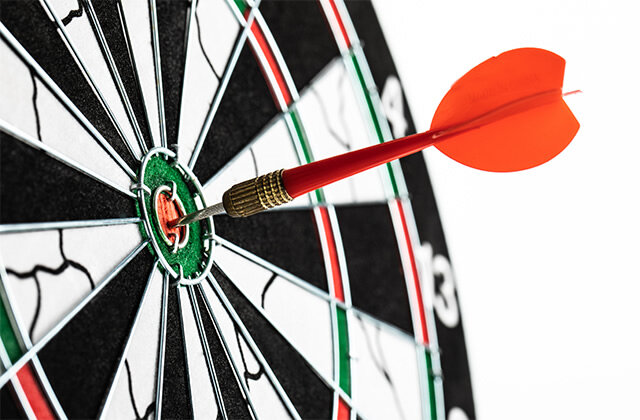
\includegraphics[width=0.5\linewidth]{asset/15582365192_640x420.jpg}
  \caption{}
  \label{fig:img21_1}
\end{figure}

几何概型实质上其实和古典概型类似, 只不过就是把古典概型从有限到无限去做了一个扩展. 它的这些特征和古典概型非常相似, 其中最不相同的就是第一点, 包含的基本事件数量无限, 第二点、第三点是一样: 

第二, 所有基本事件发生的概率均相等;

第三, 任意两个基本事件之间是互斥的;

注意一点, 即便这里包含的基本事件数量无限的, 但是所有基本事件发生的概率仍然相等. 

在这里, 就需要问大家一个小问题了, 在区间0-1这个区间里面让你们任意抽一个实数, 问, 每一个实数, 就是位于这个范围内$0-1$之间的每一个实数, 被抽中的概率是几?

正确答案是0, 这个是一个比较违反直觉的事情. 因为按照这个概率理解来说的话, 如果一个事件这个概率对应的是0的话, 我们就把它称为不可能事件. 但是很显然, 我们是可以从这个0到1之间抽一个数出来的. 竟然能被抽出来, 它的概率之前就是0. 这是很令人费解的一件事情. 

怎么样去理解这件事情呢?这个我说个题外话, 这个东西和测度论有关, 测度论可以解释为什么任意一条线上面点是无数的, 为什么任意一个面上线段的数量是无限的. 

其实测度论简单的来说就是告诉我们, 其实这个线条的长度, 或者说一个线段的这个长度不是靠这个线段上面这个点堆起来的, 是这个线段本身才有的这些性质. 当然这是一个题外话, 不是咱们课上面的一个重点. 

接下来, 我们来看一下几何概型的一些应用场景. 首先, 几何概型用于一些不规则形状面积的测量. 

比如, 我有个不规则的一个木板, 想测它的面积. 这个木板不是一个规则图形, 我们也没有什么面积公式, 那我们怎么办?我们就把它放在一个正方形的区域里面, 然后往这个区域里面去撒豆子, 把这个豆子铺满这一层. 然后我们再数, 落在这个不规则木板上面的这个豆子占豆子总数是多少. 然后, 这个比例一求出来刚好就对应着不规则木板面积和正方形区域的一个面积之比, 通过这种方式就可以把面积给算出来. 

还有一种问题是相遇问题, 相遇问题我们一样通过一个例子来看: 

一个女生和一个男生约着晚上7点到8点见面, , 如果女生先到了那他会等男生10分钟, 过时不候;如果男生先到了, 会等女生20分钟, 也是过时不候. 那为啥这个两个不公平?别问, 尊重女性. 那现在问题来了, 求他们见面的概率是多少?

如果这道题不去想用一些什么几何概型的方式去做, 是不是觉得有点头大?好像没办法去去判断. 

一个等10分钟一个等20分钟, 连这个问题怎么样解决可能思路都不太好理. 对于这种问题几何概型这种非常简单的概率模型给我们提供了一个很好的思路. 比如我们先设女生迟到的分钟数是x分钟, 男生迟到的是y分钟. 那他们能见上面的情况就是应该是: $0 \le y-x \le 10, \quad 0 \le x-y \le 20$

按照图形表示的话, 就是图\ref{fig:img21_2}: 

\begin{figure}[ht]
  \centering
  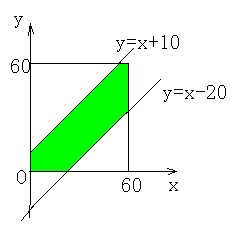
\includegraphics[width=0.4\linewidth]{asset/20230916204154.png}
  \caption{}
  \label{fig:img21_2}
\end{figure}

对应着这个图中的高亮部分, 这两条线围在一起围成了这么一个区域. 

他们两个人所有相遇的情形构成的这个正方形是一个完整的事件空间. 就是说这个x对应着男生迟到情况, y对应着女生迟到的情况, 它们俩之间相互是独立的. 也就是迟到x分钟和迟到y分钟, 两个没有任何关系, 不会相互影响. 所以, 它们整个会形成这个正方形的面积形成一个整体. 

这个正方形里面的任何一点都对应着他们的一种相遇情况, 如果说男女两人都迟到了60分钟, 在这种情况下成功约会的一个概率怎么样去计算呢?首先就是把这个整体的面积求出来, 60*60, 然后再减去这两个小三角形的面积. 被这个整体一减剩下的就是高亮部分的面积, 根据几何概型的这个思想, 高亮部分的面积除以总体的面积, 就对应着成功约会的概率. 

\begin{align*}
  P(\mbox{成功约会}) & = \frac{60 \times 60 - 0.5 \times 50 \times 50 - 0.5 \times 40 \times 40}{60 \times 60} \\
  & = \frac{1550}{3600}
  = \frac{31}{72}
\end{align*}

经过计算发现这个概率是$31/72$, 然后我们能得结论, 如果迟到20分钟见面的几率呢就低于一半了, 因为一半的话是$36/72$,在这里是$31/72$,所以我们要吸取教训, 不要以为迟到个十几、二十分钟是一个很小的事情, 约会不易, 且约且珍惜, 不要迟到. 

\section{联合概率}

好了那我们再来看一下曾经在导论课里面也上到过的一些概念: 「联合概率」, 联合概率是代表了两个或者多个事件同时发生的一个概率. 那他用符号来表示的话,就是用这个$P(AB)$或者$P(A,B)$. 

A, B两个如果是相互独立的事件, 就是说A对B没影响,B对A也没影响的话, 这个很简单, 就是把他们各自的概率给乘一块就行了:$P(AB) = P(A)P(B)$

那如果是两者并非相互独立的事件, 那我们这个时候就得一个一个看, 看哪一个事情先发生, 如果说B事件先发生, B事件发生的前提条件A发生的概率是多大. 这个就是我们待会要讲的「条件概率」, 两个乘在一起就对应的这两个非相互独立事件的一个联合概率: $P(AB) = P(A|B)P(B)$. 

给大家举了一个比较有趣的例子, 办公室的人数达到多少人, 至少有两个同事的生日一样的概率大于0.5. 

按照常规的想法, 那是不是得找365人, 需要几百号人去了. 因为刚才也说了, 生日是在哪一天是一个古典概型, 一个人的生日是任何一天的概率都是相等的, 对你而言, 你不是一个全局信息的掌控者, 没有上帝视角,所以你第一次见到这个人你会觉得他的生日在365天里面的任何一天都是相等的. 现在我们来看, 这个办公室里面人数要达到多少, 这么多同事里面最低最低还有两个人生日一样的概率是超过一半的. 

这个问题我们要怎么去看?

我们首先来考虑一下, 它的对应的反面的情形. 因为它本身题目描述的是至少有两个生日相同, 那它的反面就是说每个人的生日都不同的概率. 

我们先来考虑某一个员工甲, 第一个同事和他生日不同的概率大概就为: $364/365$.

因为甲的生日是已经确定了, 那这个同事和他的生日不同就只能从剩下的364天里面去选, 所以概率是$364/365$. 

第二个同事和前面两个人生日不同的概率是363/365,以此类推,第n个同事和前面所有人生日不同的概率推测出来就是 365-N/365. 所以所有n个员工他们生日彼此不同的概率依据联合概率的规则, 就可以写成如下这种式子: 

\begin{align*}
  P = \frac{364}{365} \times \frac{363}{365} \times ... \times \frac{365-N}{365} \le \frac{1}{2} 
\end{align*}

我们最后通过计算可以发现, 当有23人的时候, 这个办公室里面至少有两个同事, 生日相同的概率就超过了$1/2$. 因为这个计算数值比较大, 就不去给大家去做这个具体的计算了, 回头大家有兴趣自己可以去算一下. 

结论和我们之前预想的结果是不是相差特别大?因为我们之前想的是这办公室的人数至少肯定是得几百人了两个同事生日一样的概率才能大于$0.5$. 现在其找出来的情况只要有23个人, 这群人里面至少有两人生日相同的概率就过$1/2$了. 所以, 学习概率有一个好处就是, 能帮我们破解一些生活当中的不正确的一些直觉. 

\section{条件概率}

说完了联合概率, 再来说一下条件概率. 

条件概率就是当事件B已经发生的前提下, 事件A发生的概率. 符号表示为: $P(A|B)$. 

已发生的事件写在直线的右边, 还未发生要研究的事件写在左边, 这个就是它的符号表示. 

现在有这么一个问题, 条件概率描绘的是B发生的前提下A发生的概率, 那A和B不都是发生的吗?和联合概率的$P(AB)$不应该是一样的吗?$P(AB)$的描述是说A和B都发生的概率, 那$P(AB)$和$P(A|B)$有什么样不同呢?

如果我们单纯看字面意思确实是这样子的,因为条件概率说的也是B已发生, 再看A发生的概率. 那确实A和B都是发生的, 这和联合概率描述似乎是一样的. 但是他俩肯定是不一样的东西, 形式上都不一样. 那他们究竟不一样的点在于哪里呢?

两者的“外部环境”不一样;在条件概率的情形下, 我们把事件B的发生当做一件已经确定的事, B先已发生了, 然后再看A在此情形下发生的概率, 所以其概率在计算$P(A|B)$时视作1. 

因为已经发生了, 就是确定的事情了. 那既然发生了, 已经当作1了, 他对A发生有什么样的影响?可能产生的影响在于B这件事情和A是有关的, B发生了之后, A发生的情况也会产生一些变动. 

比如说, B代表了某一个学生成天是否认认真真学习, 还是成天去网吧然后熬夜, 不同的B对应的不同的A, A在这里是期末考试的成绩. B虽然是已经确定了, 但是确定了之后客观条件下就对A产生一个不可逆转的影响. 天天学习跟天天去网吧, 这两个肯定是不一样的. 所以, 在这种情况下要计算$P(A|B)$的话, 说A和B都是发生的,只不过$P(B)$在这里我们是把它发生的概率作为一个大环境已经确定的事情, 它就是1了. 

而在联合概率的情形下, 没有哪个事件先发生的说法, 没有先决条件, 既关注一个事件发生的概率, 也关注其它事件发生的概率. 联合概率是两个事件发生的概率都得参考. 在这种情况下B不是一个确定的已经得到的信息, 它不属于我们所说的这种外部环境. 

$P(AB)$和$P(A|B)$的区别就在于这里. 

\section{随机变量}

随机变量比较简单, 我们导论课内也提到过. 

一次随机试验可能出现的结果的一种数量化的表示. 

就比如我们在街上随机采访一个人, 这个人的性别本身只有男和女. 男和女本身不是一个数量化的表示, 但是我们可以把它做一个映射, 男对应着1, 女对应着0, 用数字来表示. 然后我们就可以用随机变量的这种方式去代表它, 做一些数学运算. 

随机变量一般是用大写字母去表示的, 比如X, Y. 

举个例子, 抛两个骰子得到的向上点数之和就是一个随机变量. 而且随机变量它也分两类, 一类是连续型的, 还有一类呢是离散型的. 

刚才咱们举例中, 随机采访男女身高, 身高就是随机变量. 

而离散型呢, 就是我们采访过程中的性别, 他最多就是有有限个, 不可能说是有连续多个, 它并不是稠密的. 

关于随机变量呢, 也确实也就这么多内容, 知道几个相关定义就OK了. 重点在于理解这些定义, 而不仅仅是知道怎么读. 
